\documentclass[a4paper, 12pt]{article}
\usepackage[utf8]{inputenc}
\usepackage{graphicx}
\graphicspath{ {images/} }
\usepackage[a4paper,left=1.5in,right=1in,top=1in,bottom=1in]{geometry}

\usepackage{tikz}
\usetikzlibrary{positioning,shapes,fit,arrows}
\definecolor{myblue}{RGB}{56,94,141}
\usepackage{fancyhdr}
\usepackage{booktabs}
\usepackage{mathtools}
\usepackage{amsmath}
\usepackage{etoolbox}
%\apptocmd{\thebibliography}{\csname phantomsection \endcsname \addtocontentsline{toc}{chapter}{\bibname}}{}{}
\usepackage{caption}
\usepackage{float}
\floatstyle{boxed} 
\restylefloat{figure}
\pagestyle{fancy}
\fancyhf{}
\fancyhead[LE,RO]{\footnotesize \center Comparative Study of Different Data Compression Algorithms }
\fancyfoot[CE,CO]{ \raggedright{P:F-SMR-UG/08/R0} }
\fancyfoot[LE,RO]{\thepage}

\begin{document}
 
\begin{titlepage}
    \begin{center}
        \vspace*{1cm}
        
        \large
                \textbf{Pune Institute of Computer Technology}	
                \linebreak
		\textbf{Dhankawadi, Pune}
        \vspace{0.5cm}
                        \linebreak
                        \linebreak
        \textbf{A SEMINAR REPORT }
        \linebreak
        \textbf{ON }
        \linebreak
        \vspace{0.5cm}
        \large
        \\Comparative Study of Different Data Compression Algorithms
        \linebreak
        \linebreak
		
		%\vspace{0.2cm}
		\textbf{SUBMITTED BY}
		\vspace{1cm}
		
        \textbf{ Rajat Rajesh Minekar }
        \\ Roll No. 31448
        \\ Class TE-4
        \linebreak
        \linebreak
		        
        \textbf{\large{Under the guidance of}}
		\linebreak
	    Prof. P.P.Joshi
		\linebreak
      %  \vfill
        
        
        
        \vspace{0.8cm}
        

        
\includegraphics[scale=0.6]{pict}   
        
        \Large
        DEPARTMENT OF COMPUTER ENGINEERING\\
%        \textbf{Pune Institute of Computer Technology}	
%		\textbf{Dhankawadi, Pune}
%		\linebreak
		\textbf{Academic Year 2020-21}
        
    \end{center}
\end{titlepage}
\pagebreak
%2
\begin{titlepage}
\begin{center}
	
\includegraphics[scale=0.6]{pict} 
	\linebreak
	\Large
        DEPARTMENT OF COMPUTER ENGINEERING\\
        \textbf{Pune Institute of Computer Technology}
		\linebreak
		\textbf{Dhankawadi, Pune-43}
		\vspace{0.8cm}
		\Large
		
	    \textbf{CERTIFICATE}
	    		\linebreak
	    \linebreak
		This is to certify that the Seminar report entitled
        \linebreak
		\linebreak
		\large
		\textbf{“Comparative Study of Different Data Compression Algorithms”}
		\linebreak
		\linebreak
		Submitted by
		\linebreak
		Rajat Rajesh Minekar \hspace{10mm}   Roll No. 31448 \linebreak
		\linebreak
		has satisfactorily completed a seminar report under the guidance of Prof. Rajesh B. Ingle  towards the partial fulfillment of third year Computer Engineering Semester II, Academic Year 2020-21 of Savitribai Phule Pune University. 
		\linebreak
		\linebreak
		\linebreak
		\linebreak
		\linebreak
		\begin{table}[h]
		\begin{tabular}{ccc}
		Prof. P.P.Joshi    &                        &  \hspace{52mm} Prof. M.S.Takalikar\\
		Internal Guide      &                     &    \hspace{52mm} Head \\
		          &                         &       \hspace{47mm} Department of Computer Engineering \\
                    &                       & \hspace{52mm} 
		\end{tabular}
		\end{table}
		\end{center}
Place:\\
Date:

\end{titlepage} 

\pagenumbering{Roman}
\section*{ACKNOWLEDGEMENT}

\hspace{0.5cm} I sincerely thank our Seminar Coordinator Prof. B.D.Zope and Head of Department Prof. M.S.Takalikar
for their support.
\vspace{0.25cm}
\par I also sincerely convey my gratitude to my guide Prof. P.P.Joshi, Department of Computer Engineering for his constant
support, providing all the help, motivation and encouragement from beginning till end to make this seminar a grand success.
\vspace{0.25cm}
\par 

\newpage
\tableofcontents

\newpage
\listoffigures

\newpage

\section*{Abstract}
Data Compression is regarded as the technique used to minimise data size. That is the method used to encode data in fewer bits in a smaller scale than the real size of the data. Compression is essentially technology which is used to display data without reducing quality but reducing data quantity. Compression technique was developed in order to store and transfer the data effectively. Data compression techniques like loss compression and lossless compression are available. This workshop aims at analysing and comparing these compression algorithms. It also contains multiple compressions of various data types.
\par
\section*{Keywords}
Data compression, lossy compression, lossless compression, Compression Ratio ,
Huffman, LZW, RLE, ASRL, JPEG.
\newpage
\pagenumbering{arabic}
\begin{center}
\section{INTRODUCTION}
\end{center}
\par
The Internet is a network where data flows communicate. Nowadays a lot of data is being produced every day because of technological evolution. Billions of people make use of internet and it's a huge thing to handle this growing number of results. Internet not concerned only about data but also about speed. The data flow has to be rapid to meet these requirements. Speed of 
flow increases with a decrease in data size without reducing accuracy as data is compressed.
 \\ 
\par Data are approximately 40+ zettabyte (ZB) around globally by 2020, where 1 zettabyte is 2 to power 70 bytes. Store, manipulate and flow data over a large network must be as effective as possible, when this is achieved by compression. Compression means encoding data in smaller pieces from actual dimension. Study on compression of data started in around 1940s. Robert Fano and Claude Shannon also systematically discovered a way to allocate codewords dependent on block probabilities around 1949. The ideal method for that was developed by David Huffman in 1951. Compression methods rely on encoding techniques like Run Length Encoding, Huffman encoding, etc.
\\

\par Techniques for compression decreases data size, which stored and distributed through a low bandwidth channel. The two types of compression methods are lossless and lossful. Lossless methods of compression do not lead to data or information loss, as the name suggests. The file is compressed by less bit, which means that no information is lost. This can be done using a span of mathematical and computational techniques, including entropy coding, often used to transform the file to be compressed back into its uncompressed original form. Lossless compression techniques are helpful in compression of files where entire info should be preserved, such as executable files.
\\

\par 
LZ77 and Huffman coding are often used for lossless encoding systems. The process of lossy compression removes unnecessary bits from a disc, which decreases their size. Since any information is lost when encoding the compressed file cannot be returned to the original file. The decompressed file is a similar proximity to the original file that is recovered with the understanding of the compression application. Loss-based compression techniques have a higher compression rate than loss-free compression techniques so more redundant data are removed. We equate different modern algorithms that are widely used without failure.
\\


\newpage
\begin{center}

\section{MOTIVATION}

\end{center}

\hspace{1cm}As we are in the digital era, our dependency on internet and electronic devices is increasing exponentially. 500 hours of video were uploaded on YouTube every minute as of may 2019, this is just a fraction of total data. Data compression needed to decrease this size to help in data storage and also in data transmission. 
 \\

  

\hspace{1cm}Data compression has became very important part of internet and it has modern techniques, views and optimizations. So, selecting proper compression algorithm is very necessary for the internet.
\\

\newpage
\begin{center}
\section{A SURVEY ON PAPERS}
\end{center}
\subsection{Modern Lossless Compression Techniques: Review, Comparison 
and Analysis}
\hspace{1cm} In this paper, We contrasted and evaluated the efficiency of current 
lossless compression algorithms. The findings of the simulation indicate that the 
compressed image that Huffman codes and run-length codes produced is almost 
the same as the initial image after decompression. The coding algorithm is basic,
but the coding ratio is very poor. This coding technique can be used where the 
consumer does not expect good image resolution and does not pay any attention 
to the compression ratio.
The author concluded that, In the case of selecting algorithms, different 
algorithms can be used for different data formats


\subsection{A STUDY ON VARIOUS DATA COMPRESSION TYPES AND 
TECHNIQUES}
\hspace{1cm}  
This paper gives an overview of different methods for loss-free compression. 
Compression is the act of altering or encoding the bits of data to reduce the amount of 
storage space. It improves the storage of one or more data instances or elements to be 
reduced. Essentially in cases where compression is required where the reconstruction 
is similar to original compression algorithms are most needed.
Author concluded with overview of Different type of techniques for compression on 
different types of data such as image, text, audio, etc.



\subsection{Research on Image Compression Coding 
Technology}
\hspace{1cm} 
This paper presents an overview of the many compression methods on the image without loss.
Compression is the action through which bits of data are altered or encoded in order to minimise storage space. It enhances the storage of one or more data instances or pieces. Especially if compression is needed if the reconstruction is identical to the original compression techniques.
An summary of the image compressing techniques concluded the author.
\\

\newpage
\begin{center}
\section{PROBLEM DEFINITION AND SCOPE}
\end{center}

\subsection{Problem Definition}

\hspace{1.5cm} To study the of Data Compression and the different techniques used to achieve it.

\subsection{Scope}

\hspace{1.5cm} We were using the traditional compression algorithms for past years. But as we are stepping towards the future, we are dealing with emerging technologies like machine learning, data science, etc. While colluding with these technologies, we can use these technologies to make these algorithms more efficient.\\

\hspace{1.5cm}We will analyze various techniques by performance measures like compression ratios. It will be possible to evaluate the effectiveness of each algorithm and analyze its optimizations using compression ratios.

\newpage
\begin{center}
\section{Data Compression Algorithms}
\end{center}
\subsection{Data Compression:}
\par
\hspace{1cm}It is encoding data into smaller bits than it was originally. There are two kind of compression, lossless compression: one where the size of the data is reduced without affecting its quality, and the other lossy compression: where size reduction is only considered irrespective of its quality
\\
\subsection{Working Principle of Compression:}
\par
\hspace{1cm}It is carried out by a method that employs a way to decide how to reduce the data's size. The algorithm may use a dictionary to convert a string containing bits — or 0s and 1s to a smaller string of 0s and 1s, or the algorithm may insert a reference or pointer to a string containing 0s and 1s that the program has already seen. Text compression will delete all unnecessary characters, insert a single repeat character to signify a string 
containing repeated characters, and replace a frequently occurring bit string with a smaller bit string. A text file can be compressed to 50% or even a higher percentage of its original size using data compression. Compression of data content or the whole transmission unit, including header data, may be done for data transmission.Information can be sent or received through the internet in a ZIP, GZIP, or other compressed format, either individually or as part of an archive file
\\
\subsection{Data compression types: lossless and lossy compression}
\textbf{Lossless Data Compression:}
\par To enable the exact data to be taken from the compressed data, lossless compression takes help of algorithms for compression. Lossless compression in contrast to lossy compression, which does not allow for the exact reconstruction of the actual data from the compressed one. Where it is necessary that the actual and decompressed data could be similar, or where no determination can be performed if a particular deviation is uncritical, use of lossless compression takes place. When a file is in original state, Lossless compression allows it to get restored in its actual state without losing a single bit of data.
When it comes to executable files, text and spreadsheets, where the loss will 
change the details, lossless compression is common technique. Lossless compressions may be classified based on the format of data to be compressed. Text data, executables data, jpeg data, and mp3 formatted data are the most commonly taken by compression methods. The majority of lossless compressions are of two kinds of algorithms: one which creates a statistical model for the inputs, and another that maps inputs to the bits of strings by this model, with "probable" data producing shorter output than "improbable" one.
\\
\textbf{Lossless compression algorithms:}
\par
1. The Huffman coding
2. Arithmetic coding
3. LZW
4. Run Length Encoding (RLE)

\subsection{Entropy coding}
\par
\hspace{1cm}In entropy encoding method codes assigned to symbols to fit code lengths to symbol 
probabilities. In general, entropy encoders compress the data by doing replacement of
symbols represented by equal-length codes with symbols represented by codewords 
whose length to be proportional with probability's negative logarithm. Huffman and 
arithmetic encodings are two most widely used which are entropy based encoding methods. 
\\

\subsection{Huffman coding }
\par
\hspace{1cm}This coding is a lossless compression method based on entropy. Making use of a 
variable length code table to encode a source, like character as in file, where the 
variable-length code has been extracted in a specific way based upon 
approximate occurrence for every value of the source possible, is referred to as this 
technique. The Universal Huffman Tree based encoding, it is novel and efficient text 
compression method that compresses any word level text in a universal manner for 
corpora across domains. The work's main contribution is the avoidance of code table 
contact during the decoding. We can compact any text using Universal Huffman Tree 
without having to produce a new tree for each input, which considerably reduces the size 
of the code table.\\
\\Prefix Codes are input character allocated variable length codes. This is to 
delegate the codes in a manner where no other code of character is prefixed to the code 
allocated to one character. Huffman Coding means that the built-in bitstream is 
uncertainly decoded.
\\

\subsection{Huffman Tree Construction Steps}
\par
\hspace{1cm}
The input consists, array consisting unique characters and their number of 
appearances, while the output is a Huffman Tree
\\
\par 1. Create leaf nodes for each distinct character and a min heap of all leaf nodes (the 
Min Heap act as priority queue). To equate two nodes from min heap, value for 
frequency gets used. At first, the least common character is at position of root.)
\par
2. In min heap, take two nodes having lowest frequency.
\par 3. New internal node created with the frequency same as before as the two nodes. the 
first extracted node assigns left child, and right children to the second extracted 
node. This node to be added to a minimum heap.
\par 4. Steps 2 and 3 be repeated unless heap remains with one node. Root node becomes
last node in tree, and it completes.
\par 5. Starting on root and working our way up to tree. Maintain auxiliary array. Write 0 
to array as you moves towards left child. Write 1 to array while keep moving 
towards the right one. When leaf node gets encountered, print that array
\\

\subsection{Compression Ratio:}
\par Compression ratio for this algorithm is 1.5:1, or about 8 bits/5.32 bits\\

\subsection{Flowchart}

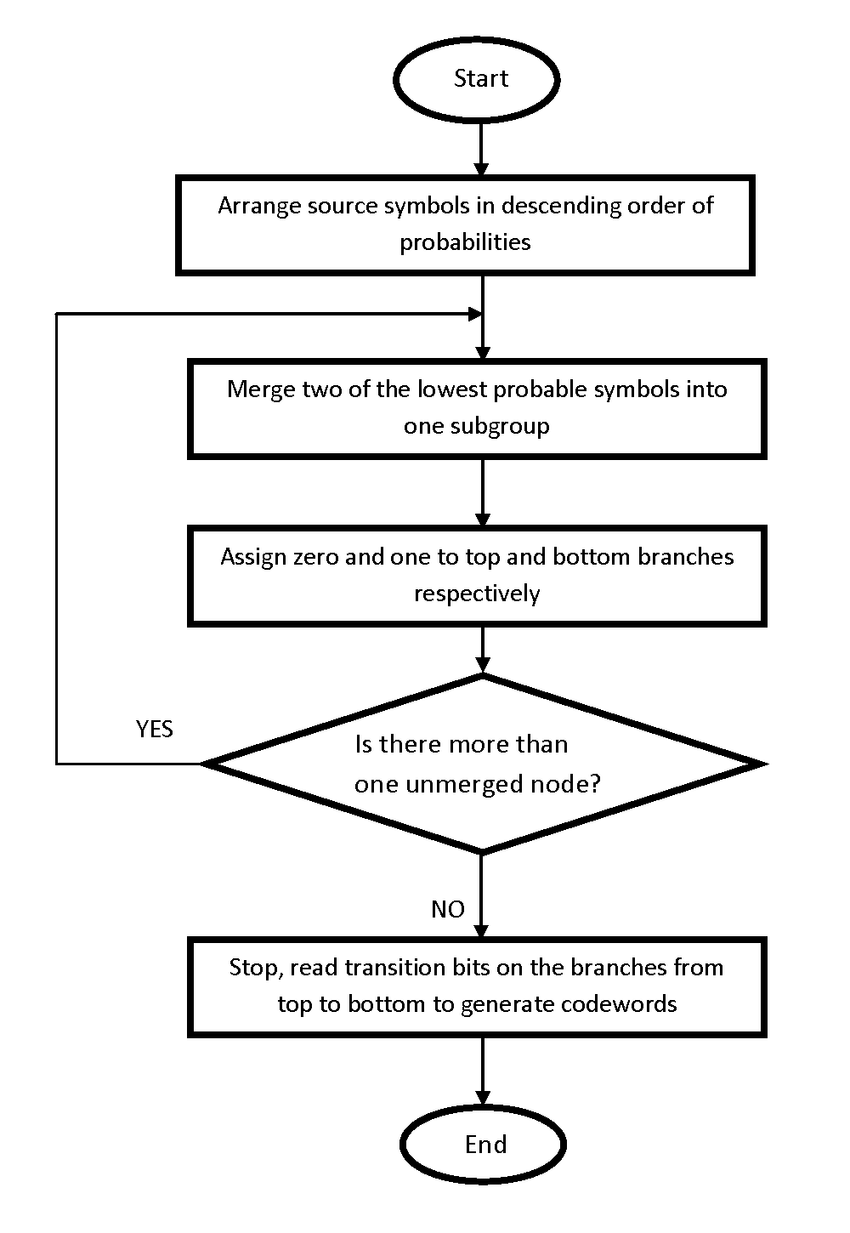
\includegraphics[scale=0.4]{Huffman-Coding-Flowchart}

\captionof{figure}{Huffman coding compression flowchart.}
\vspace{5mm}
\subsection{Time Complexity Analysis}
\par The complexity of Huffman coding is O(nlogn) since it uses a min Heap data structure 
to enforce a priority queue.
It takes O(nlogn) time to build a min heap (moving an element from the root to 
the leaf node requires O(logn) comparisons, which is achieved for n/2 elements in the 
worst case).
Building a min heap takes O(nlogn) time (moving an element from the root to 
the leaf node requires O(logn) comparisons, and in the worst case, this is achieved for 
n/2 elements).
The algorithmic complexity of the whole operation computes to O(nlogn) since 
constructing a min heap and sorting it are done in order.If the characters are already 
sorted according to their frequencies, we can use a linear time algorithm.
\\

\subsection{ Advantages:}
\par 1. binary codes produced can vary in length, this coding method saves a lot of memory space.
\par 2. To encode characters which occur more often in input, it produces short binary codes.
\par 3. There are no prefixes in binary codes that are created.
\\

\subsection{Disadvantages:}
\par 1. When opposed to lossy methods, lossless methods, like Huffman encoding
method, achieves low compression ratio. As result, lossless approaches like Huffman method are only useful for coding text and application data, not 
digital images.
\par 2. Since Huffman method use two passes, one is for constructing statistical 
model where on other hand for encoding, is slower operation. As a result, 
lossless approaches which use Huffman method are much slower than other 
methods.\\
\par 3. binary codes are different according time, hence it's difficult to decode
tools to tell if encoded data is corrupt or not. This could lead to incorrect 
encoding and, as result, incorrect performance.\\

\subsection{Applications:}
\par 1. All the compression formats using Huffman method are GZIP, PKZIP with
BZIP2.
2. For video, like PNG, JPEG, and MP3 Huffmann method is used 
3. Huffman method continues to dominate the compression market, as modern 
range and arithmetic coding schemes have been overlooked because of patent 
issues.
\\

\subsection{Example:}
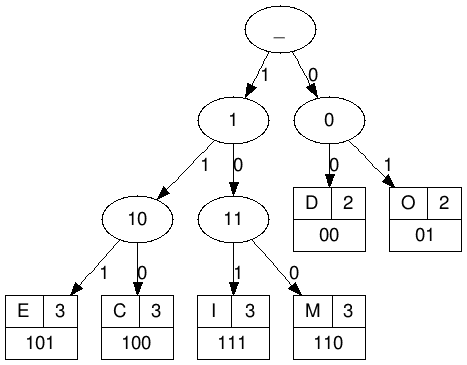
\includegraphics[scale=0.8]{huffman-tree-dcodemoi}

\captionof{figure}{Huffman coding tree creation for example text=’DCODEMOI’}
\vspace{5mm}


\newpage
\section{ Arithmetic Coding}
\par The most powerful way to code symbols is by arithmetic coding depending upon their probability. According to information theory, the typical code length is exactly as little as possible. The bit resolution of binary code trees does not cause any deviations. Arithmetical coding has a considerably higher compression rate than the binary Huffman coding tree.\\
\par  It is more complex, on the other hand, to execute it. A message is coded as a true number between one and zero in the arithmetic coding process. Arithmetic code has a higher compression ratio, in comparison to Huffman coding. Instead of many codewords, a single symbol is created.\\
\par The coding of arithmetic is a type of unlost coding. There are few disadvantages of using arithmetic coding. One is that you need to understand the whole codeword so you can decipher the symbols, because if a corrupt bit is sent into the codeword,the whole message can be corrupted. Number of symbols encodable in a codeword is constrained by the precision of the encoding number. Arithmetic coding offers certain patents, so you can pay a little for using those algorithms.\\
\par The format of the JPEG data is arithmetic-coded. It’s used as an alternative to Huffman coding for final entropy coding. In view for legal limitations above, considering their poorer efficiency, Huffman coding remains normal.
\\

\subsection{Arithmetic Coding Algorithm}
\par Arithmetic coding method works in opposing direction, from leave to root.
\par 1. Begin by splitting the range [0, 1] into subrange of every possible symbol 
that could appear in a message. Make each subinterval's size equal to how 
often it will be appearing in post.
\par 2. While encoding symbols, you will "zoom" through the current interval and 
split it in to subintervals the same as you did with new set in stage one.
\par 3. Repeat the operation until the machine's maximum precision has came or all 
the symbols have been encoded.4. For sending codeword, number is send which is within the most recent interval. Number of symbols getting encoded shall be specified in image 
format's protocol.
\\
			
\subsection{ Time Complexity}
\par Arithmetical coding techniques time complexity is O (nlogn)
\\

\subsection{Advantages:}
\par Compression ratio of arithmetic coding, it’s higher than Huffman as it uses 
a single symbol rather than several words
\\

\subsection{Disadvantages:}
\par 1. To begin symbols decoding, the whole codeword has to be obtained, and the 
whole message will get corrupt if a damaged bit exists inside the codeword.
\\
\par 2. Number of codable symbols limited to the precise number which could be 
coded is the precise number. 
\\

\subsection{ Applications:}
\par Length of codeword is similar with ideal value, which will result in greater 
compression, since the arithmetic code for VLSI testing is used.\\

\subsection{Example:}
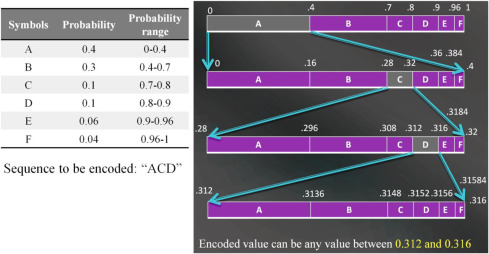
\includegraphics{arithmetic-example}
\captionof{figure}{Arithmetic coding for sequence text=’ACD’}
\vspace{5mm}


\newpage
\section{LZW(Lempel–Ziv–Welch)}
\subsection{LZW:}
\par A typical compression method is the LZW algorithm. In GIF and to a lesser 
degree, PDF and TIFF, this algorithm is widely used. The 'compress' order in 
Unix, among other stuff. It is lossless, which means during the compression 
process no data is lost. Algorithm has been simple to implement in hardware 
implementations and has good performance potential. The principle depends on 
repeated patterns to conserve data space. LZW is the technology most commonly 
used for general data compression because of its simplicity and versatility.
 \\
\par The way LZW compression functions is to read a number of symbols, arrange 
the symbols into strings and translate the strings into codes. Compression has
achieved, since the protocols have less space than the strings they replace.
\\

\subsection{ Working:}
\par 1. Code table is used for LZW compression, and number of entries in table is
commonly set to 4096. From code table, single bytes in input file are often 
allocated to codes 0-255.
\\
\par 2. Code table includes first 256 entries only as encoding starts, with remaining 
table becoming void. The codes 256 from 4095 are used to describe byte
sequence in compression.
\\
\par 3. LZW detects repetitive sequence manner in data and applies them on to code 
table to consider as encoding progresses.
\\
\par 4. Codes from compressed file is extracted and translated via code table to 
determine which character it represents.
\\

\subsection{ Advantages:}
\par 1. The algorithm for LZW compression is incredibly rapid.
\\
\par 2. The whole algorithm can be shown in just a decade without interpreting the 
incoming text.
\\
\par 3. it is an easy to use algorithm for lossless compression.
\\
\par 4. LZW shines with repeated strings when it comes to data sources. As a result, 
the compression of English text is incredibly well. At least 50 percent are 
supposed to be compressed.
\\
\par 5. The LZW algorithm operates much as designed with any fixed stationary 
source
\\

\subsection{ Disadvantages:}
\par 1. While the algorithm is simple, its implementation is challenging due to the management of the string table.
\\
\par 2. Files with no repetitive data cannot be very well compressed.
\\
\par 3. Text files perform well but not so well for other file formats. 3.
\\
\par 4. Total duration of all strings is calculated, amount storage required is not specified\\

\subsection{Flowchart:}
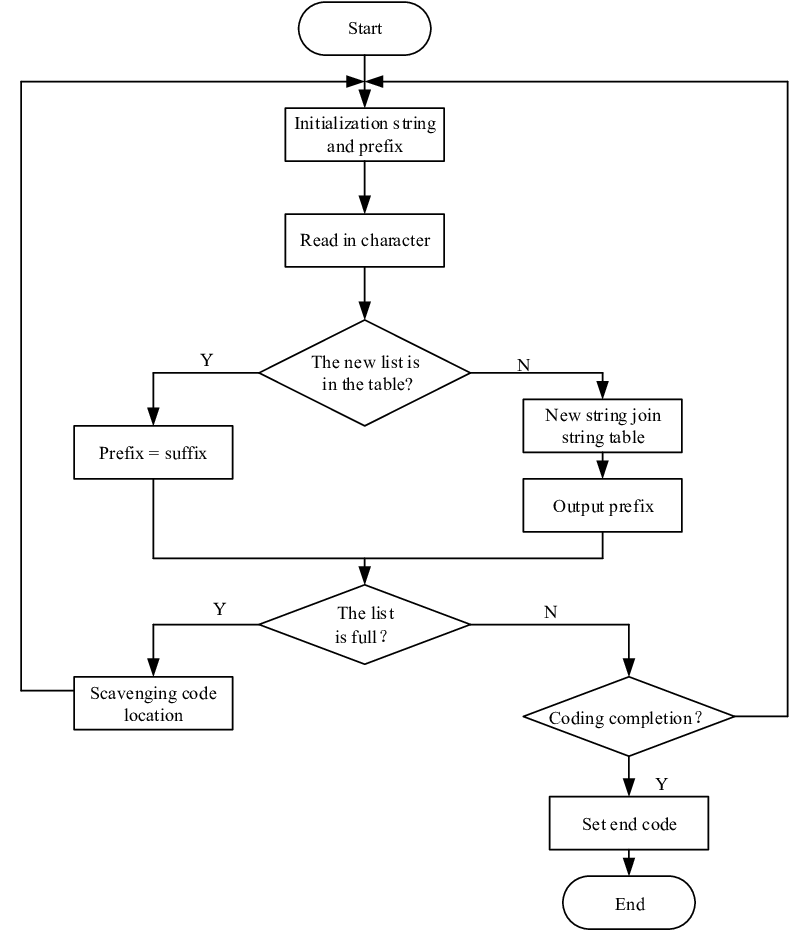
\includegraphics[scale=0.5]{lzw flow.jpg}
\captionof{figure}{LZW compression Flowchart.}
\vspace{5mm}

\subsection{Application:}
\par A common compression technique is the LZW measurement. The formula is 
used in GIF and PDF or TIFF on a daily basis.
\\
\subsection{Example:}
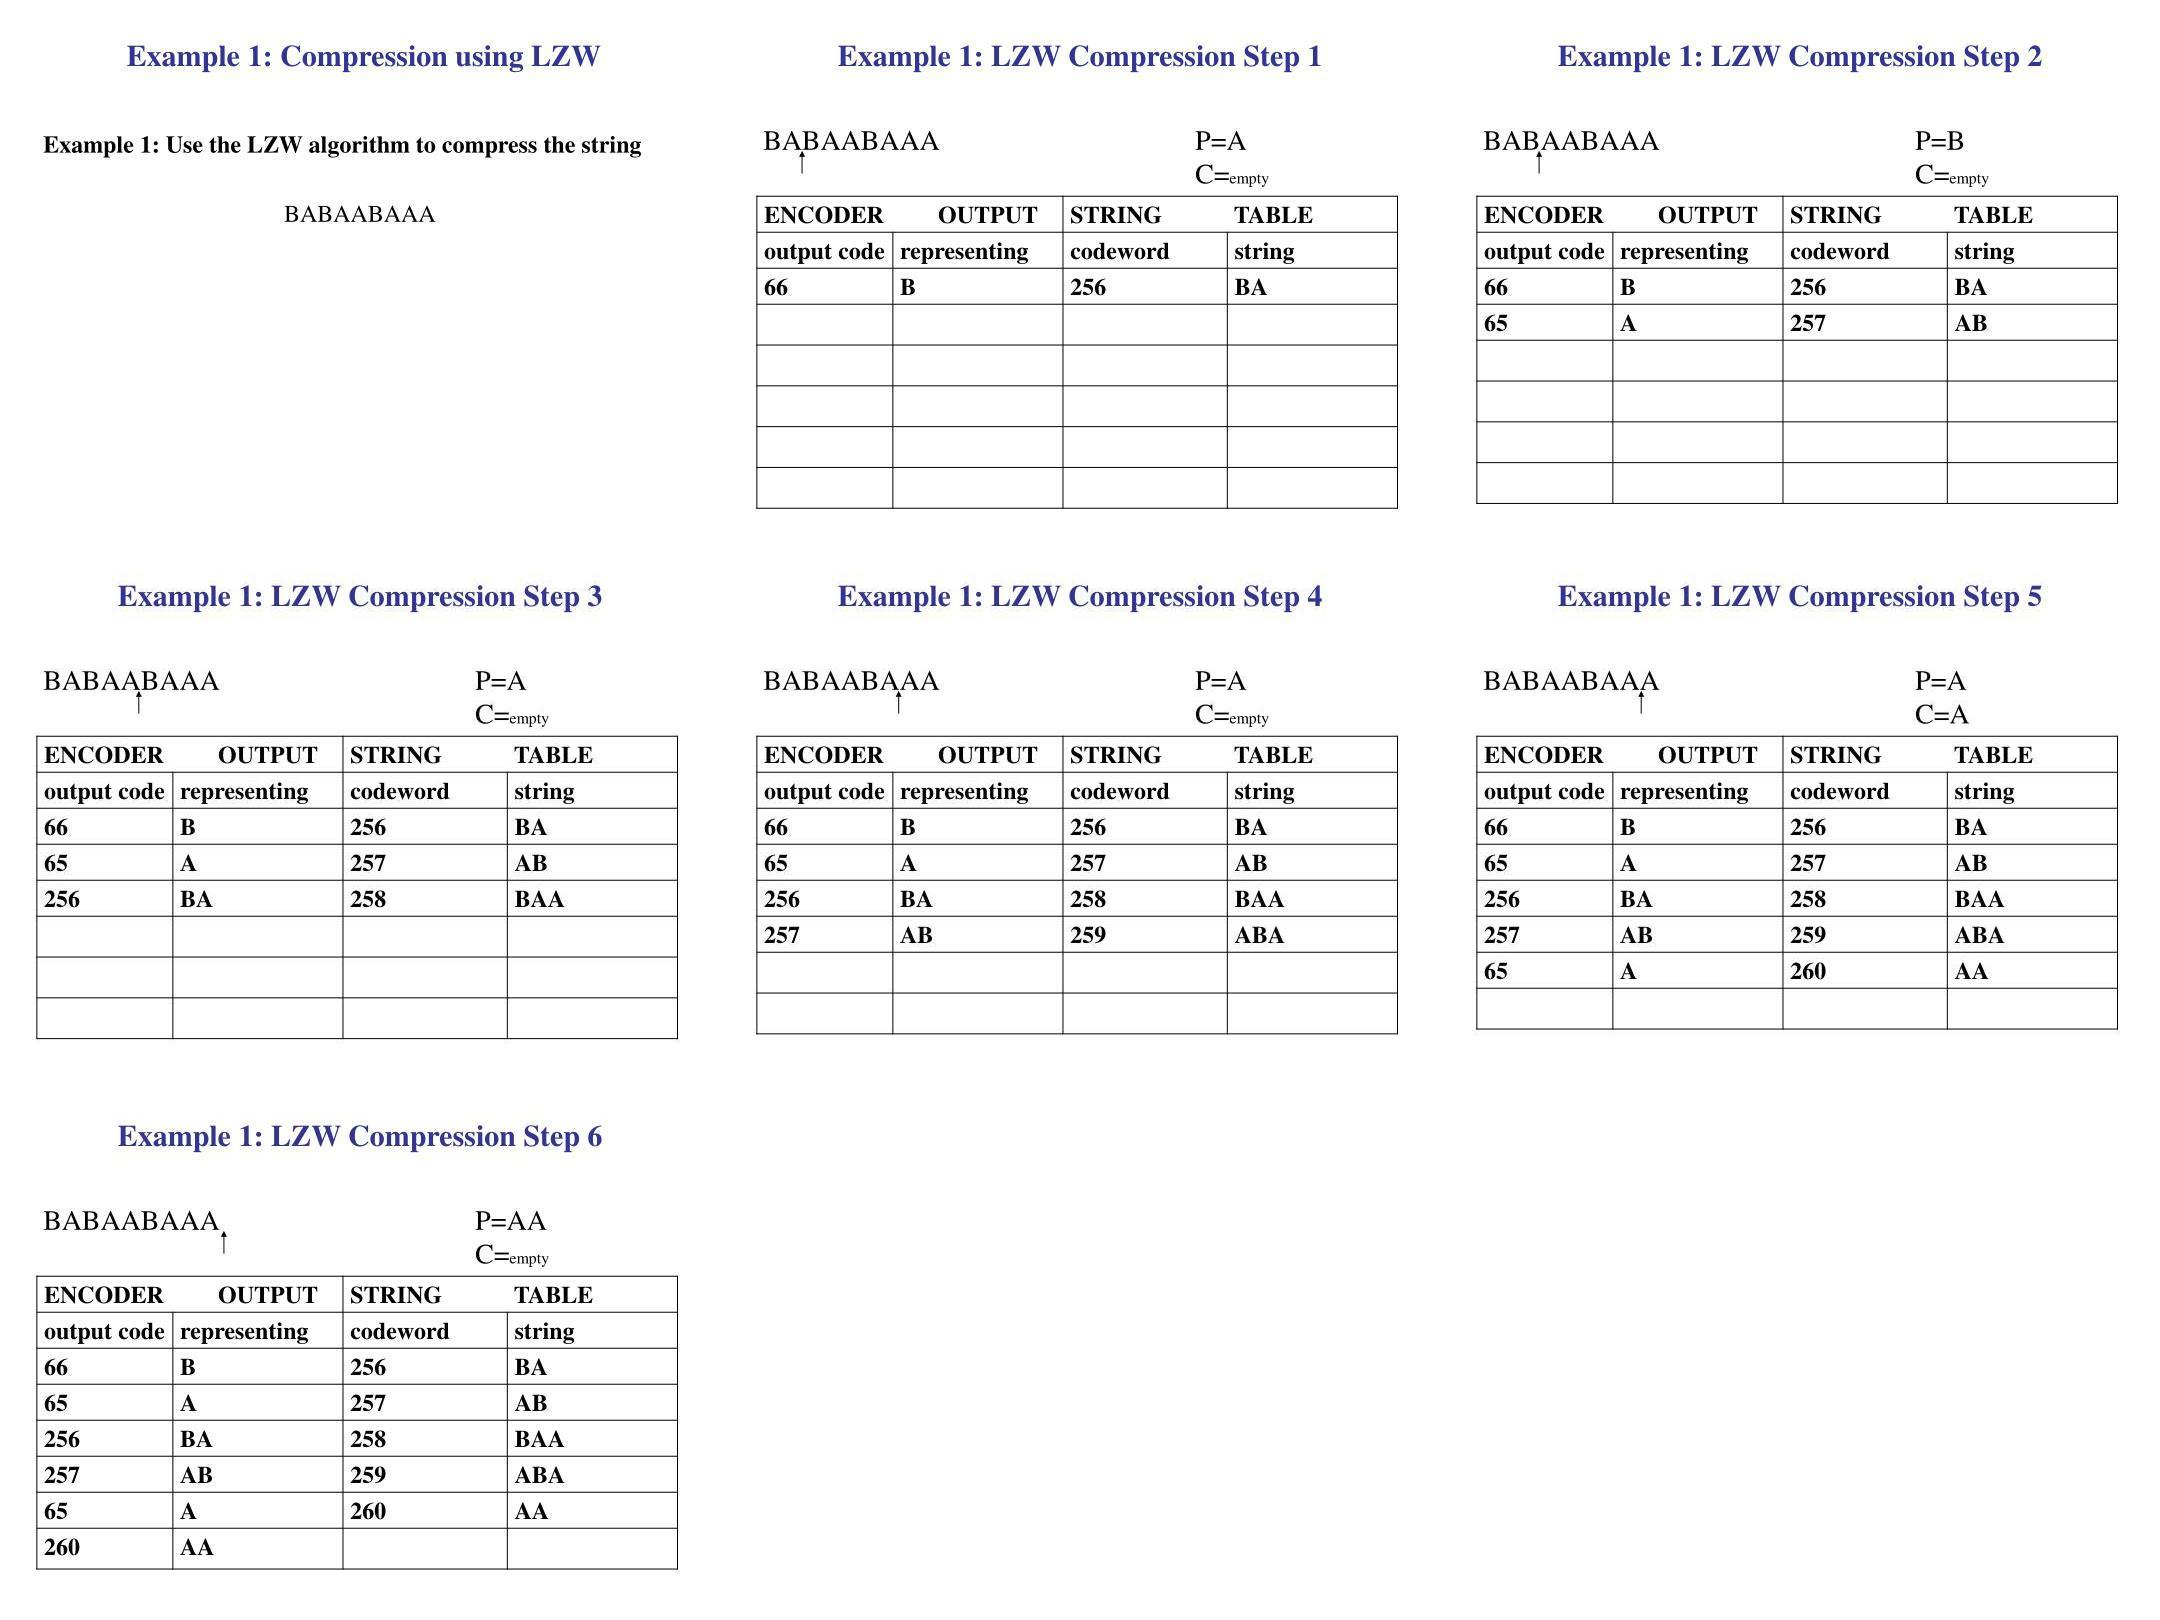
\includegraphics[scale=0.3]{lzwexample.jpg}
\captionof{figure}{LZW compression Example.}
\vspace{5mm}


\newpage

\section{Run Length Encoding}
\subsection{Run Length Encoding:}
\par Run-Length-Encoding is very easy data compression method in which data 
runs are stored instead of in the initial run as single data and number. This 
approach works well with data and contains several runs including simple 
graphics such as icons and illustrations. This approach works well.
\\
\par A several coloured blocks of similar colour usual it 
consist of image. For scanning of colour blocks, the same colour value is 
often maintained by consecutive lines or continuous pixel in same scanning 
rows. The coding run-length saves the same pixel value with number of pixel
values of similar colour instead of saving the same colour blocks one by one 
in a picture. Color values and count values are simply put to represent 
several times in a row the same colour pixel values.
\\
\par If a picture contains several colour blocks of the 
same colour, run-length coding has a high degree of compression. When the 
colour value of an image is high, the runtime of the image is low and 
runtime coding can lead to further redundancy.
\\

\subsection{Algorithm:}
\par 1. As input, take strings. \\
\par 2. In the input string count how much times an entity occurs.\\
\par 3. It is used to encrypt the frequency of the variable.\\
\par 4. Return strings as an encoding output.
\\

\subsection{Advantages:}
\par This algorithm is easy to use and requires less power from the CPU.
\\

\subsection{Disadvantage:}
\par  RLE compression only benefits files with a lot of redundant data.
\\

\subsection{ Applications:}
\par Typically RLE is used for
1. PDF files
2. TIFF file
\\

\newpage

\subsection{Flowchart:}
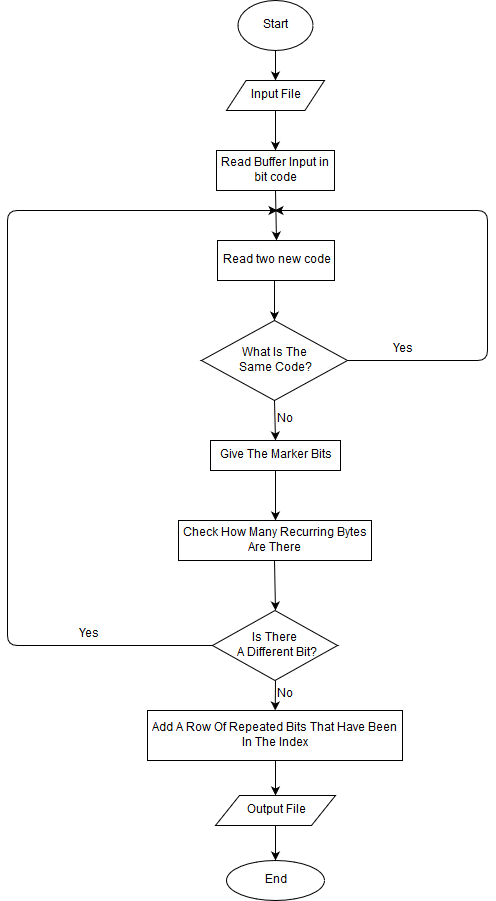
\includegraphics[scale=0.7]{Flowchart-Diagram-Compression-Data-With-RLE.jpg}
\captionof{figure}{RLE compression Flowchart.}
\vspace{5mm}

\newpage

\subsection{Example:}
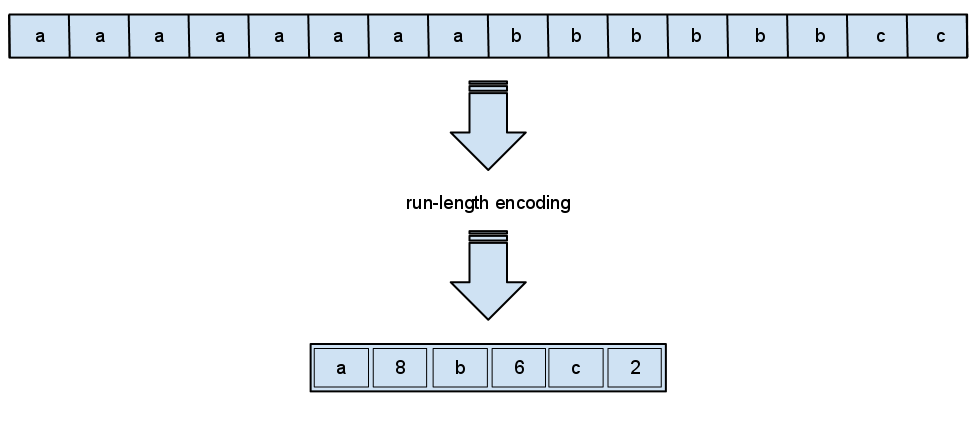
\includegraphics[scale=0.5]{Run-lengthEncoding.jpg}
\captionof{figure}{RLE Example.}
\vspace{5mm}

\newpage
\section{Lossy Compression:}
\par A data loss compression process involves the compression and 
decompression done on data, which can vary from actual but is "like 
enough" to be helpful. Lossy compression on data is used extensively on the 
Internet, in particular for media and telephony applications. Most data 
compression formats are losing generation, which results in a persistent lack 
of continuity as the file is compressed and de-compressed. In comparison to 
lossless compression on data. Loss compression method are intended for
delete outdated or duplicate records, meaning that space is saved instead of 
data integrity is maintained.
\\

\par Human experiments usually observe only minor or 
undetectable losses. Images and audio files that could be trimmed at the 
edges are compressed using Lossy compression techniques. Images and 
audio, with the exception of text and processing files, do not require 
restoration to be similar with the original, particularly if the data lost is 
minor or undetectable.
\\
\par Lossy compression permanently removes obsolete, 
insignificant, or imperceptible bits of data. Lossy compression is useful in
graphics, audio, video, and images where loss in few data bits has little to 
little impact to material representation. Lossy or lossless image encoding 
can used with graphics
\\

\subsection{ Image Compression:}
\par The difference between the large amount of data 
and the bandwidth of visual images on a narrow channel highlights the 
significance of picture encoding. The redundancy of the image relates to the 
details between pictures. In order to ensure image exactness, data compression 
must avoid replication of images. Different compression methods are usually 
used to process data to eliminate multiple types of repetition
\\

\newpage
\section{Experimental results:}

\subsection{Huffman compression on Image:}
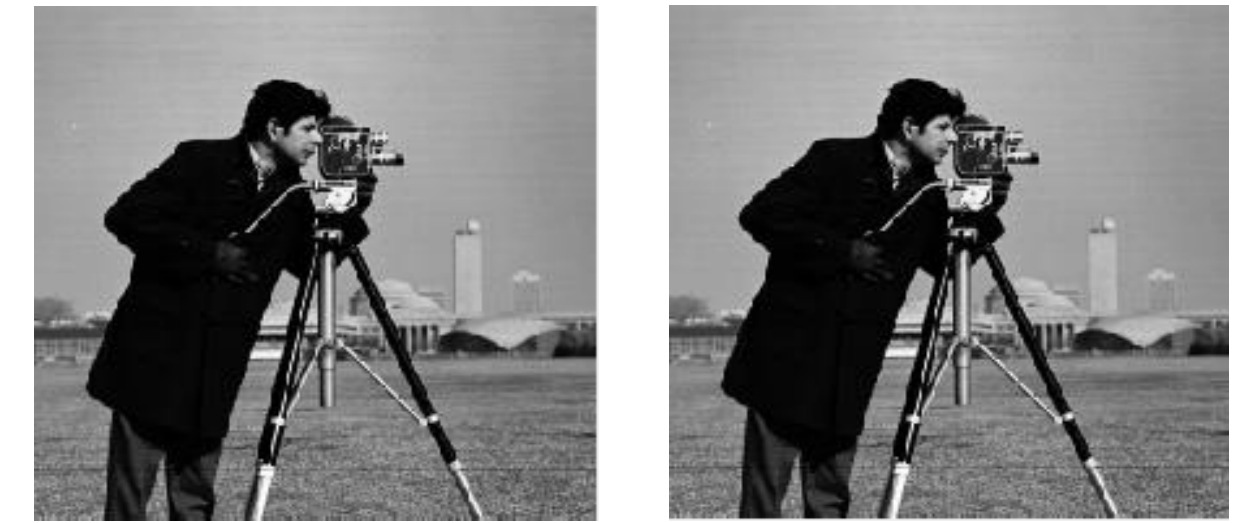
\includegraphics[scale=0.5]{huffmanImage.png}
\captionof{figure}{Compressed Image and Decompressed Image}
\vspace{5mm}

\subsection{Run Length Coding compression on Image:}
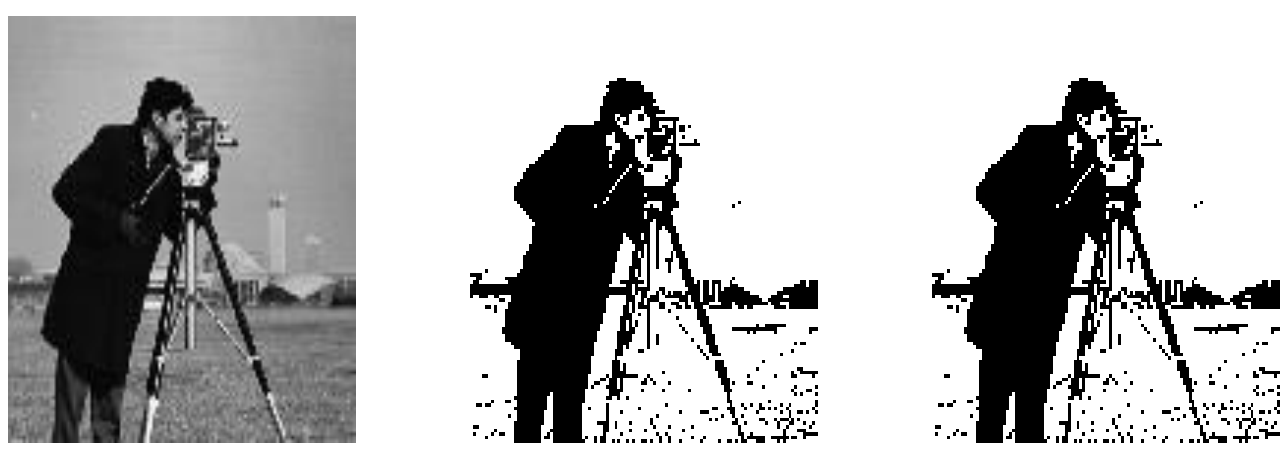
\includegraphics[scale=0.5]{rleImage.png}
\captionof{figure}{Original Image, binary image, compressed and decoded image}
\vspace{5mm}

\newpage
\section{Conclusion}
\par The advantages of compression include decreased hardware compression, data delivery 
and bandwidth and cost savings. Moreover, it takes less than uncompressed time to 
upload a compressed file and it requires less network bandwidth. An important 
downside of the data compression is the performance hit by using CPU and storage 
resources to compress and decompress data. Lossless algorithms of compression do not 
lead to data loss, as their name suggests. And if the data is compressed without loss, it 
can recovered through data compressed accurately after a while. Memory documents, 
spreadsheets, word-processing files, and even different kinds of images and videos data 
are commonly compressed using Lossless compression. The compression without loss 
is really useful in the compression of text. The restoration of the original text is crucial, 
because even small variances lead to phrases with various meaning.
\\
\par We have learned various algorithms, such as Huffman encoding, RunLength-Encoding, LZW Compression, etc. We also analyzed and worked on these 
algorithms. We also found that Huffman coding used worldwide norm algorithm and 
that the correct compression algorithm should be chosen for efficacy according with
data formats
\\


\newpage
%
%\bibliography{biblio}
\addcontentsline{toc}{section}{References}
\bibliographystyle{plain}

\begin{thebibliography}{21}
\bibitem{paper1} K.Muthuchamy ,“A STUDY ON VARIOUS DATA COMPRESSION TYPES AND TECHNIQUES”, VOLUME 5 I ISSUE 3 I JULY – SEPT 2018.

\bibitem{paper2} Oswald, C and Sivaselvan, B. 2018. Text and Image Compression based on Data Mining Perspective. Data Science Journal, 17: 12, pp. 1–12.

\bibitem{paper3} Linglong Tan, Yong Zeng* and Wenju Zhang , “Research on Image Compression Coding Technology” , IOP Conf. Series: Journal of Physics: Conf. Series 1284 (2019) 012069.


\bibitem{paper4} S.Anandhi, R.Neela, M.Janaki Rani , “Efficient Test Data Compression for SoC through ASRL with Improved Dictionary based Compression Technique” , IJITEE, ISSN: 2278-3075, Volume-8 Issue-11, September 2019


\bibitem{paper5} Apoorv Gupta, Aman Bansal , Vidhi Khanduja , “Modern Lossless Compression Techniques: Review, Comparison and Analysis” , Conference: 2nd IEEE International Conference on Electrical, Computer and Communication Technologies (ICECCT - 2017) At: Coimbatore, India ,Volume: 3.



\bibitem{paper6}M. Goyal, K. Tatwawadi, S. Chandak and I. Ochoa, "DeepZip: Lossless Data Compression Using Recurrent Neural Networks," 2019 Data Compression Conference (DCC), 2019, pp. 575-575, doi: 10.1109/DCC.2019.00087



\bibitem{paper7} Khairi, Nor & Jambek, Asral. (2017). Study on data compression algorithm and its implementation in portable electronic device for Internet of Things applications. EPJ Web of Conferences. 162. 01073. 10.1051/epjconf/201716201073.


\end{thebibliography}


\newpage
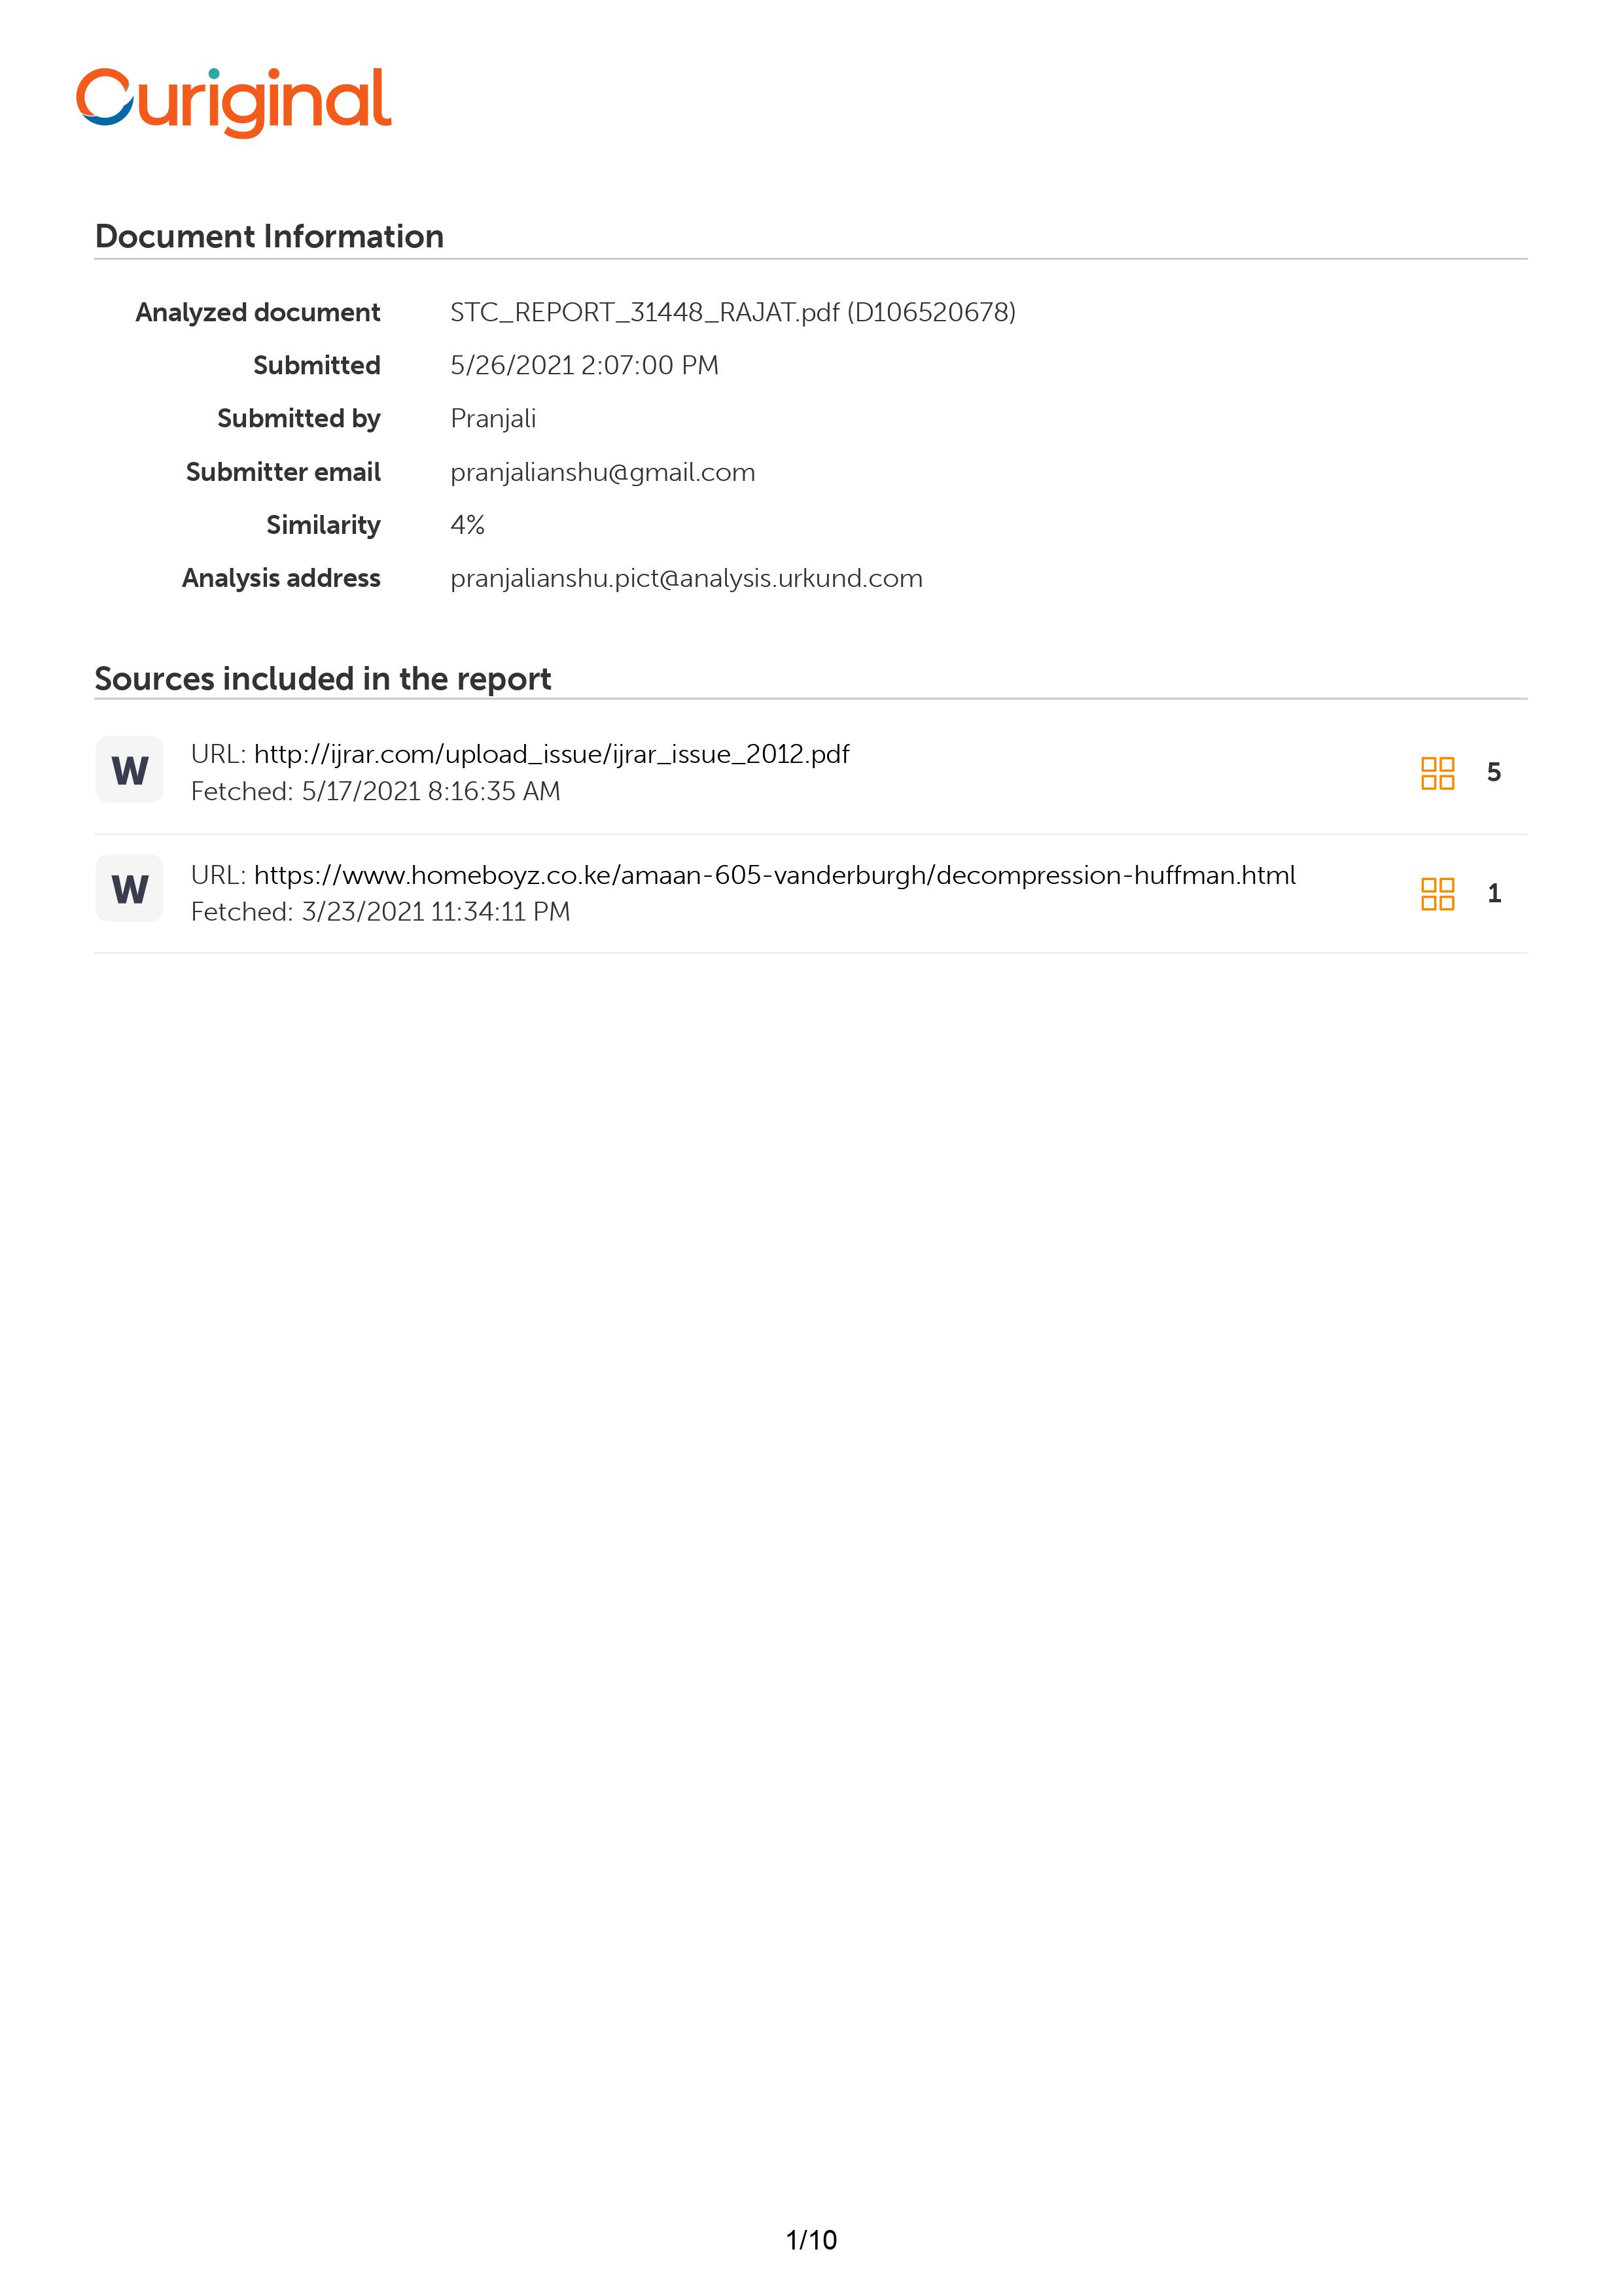
\includegraphics[scale=0.8]{plag.jpg}
\vspace{5mm}

\newpage
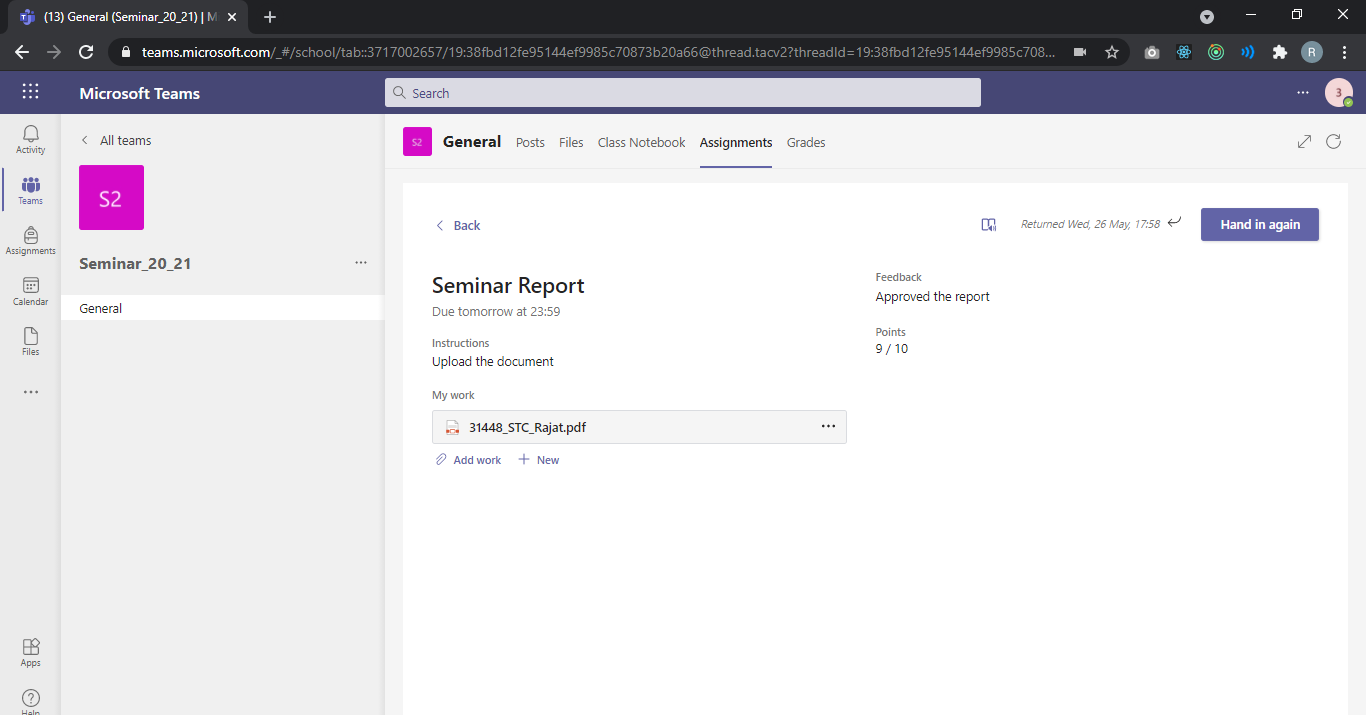
\includegraphics[scale=0.4]{approve.png}
\vspace{5mm}


\end{document}

